\QCMautoevaluation{Pour chaque question, plusieurs réponses sont proposées. Déterminer celles qui sont correctes.}

\begin{QCM}
\begin{GroupeQCM}

\begin{exercice}
Les équations sont :
\begin{ChoixQCM}{4}
\item $A = 3x + 4$
\item $5x^2 + 6x - 3 = 0$
\item $6a + 1 = a - 2$
\item $6y + 7$
\end{ChoixQCM}

\begin{corrige}
\reponseQCM{a}
\end{corrige}
\end{exercice}



\begin{exercice}
$x = -3$ donc...
\begin{ChoixQCM}{4}
\item $4x > 0$
\item $2x + 5 = \dfrac{2x}{3}+ 1$
\item $x^2 + 6x + 9 = 0$
\item $x + 7 = - 21$
\end{ChoixQCM}

\begin{corrige}
\reponseQCM{a}
\end{corrige}
\end{exercice}



\begin{exercice}
$-8$ est la solution de l'équation...
\begin{ChoixQCM}{4}
\item $2a + 17 = 1$
\item $(8 + x)(x + 3) = 0$
\item $0x = 0$
\item $n^2 = 64$
\end{ChoixQCM}

\begin{corrige}
\reponseQCM{a}
\end{corrige}
\end{exercice}



\begin{exercice}
$3x - 4 = -2x + 11$ donc...
\begin{ChoixQCM}{4}
\item $-1x = 9x$
\item $5x = 7$
\item $x = 3$
\item $5x - 15 = 0$
\end{ChoixQCM}

\begin{corrige}
\reponseQCM{a}
\end{corrige}
\end{exercice}



\begin{exercice}
L'équation $2x - 6 = 2(-  + x)$...
\begin{ChoixQCM}{4}
\item admet 0 pour solution
\item n'a pas de solution
\item a les mêmes solutions que $0x = 2$
\item est impossible
\end{ChoixQCM}

\begin{corrige}
\reponseQCM{a}
\end{corrige}
\end{exercice}



\begin{exercice}
$4a + 5 = a + 15$ donc...
\begin{ChoixQCM}{4}
\item $3a = 10$
\item $a = 1,3333$
\item $a = 4$
\item $a =\dfrac{3}{10}$
\end{ChoixQCM}

\begin{corrige}
\reponseQCM{a}
\end{corrige}
\end{exercice}





\begin{exercice}
\og Le double de la somme d'un nombre et de 3 est égal à la moitié de ce nombre, augmentée de 5 \fg
\begin{ChoixQCM}{4}
\item $\dfrac{x}{2} + 3 = 2x + 5$
\item $2x + 3 = \dfrac{x}{2}+5$
\item $2(x + 3) =\dfrac{x+5}{2}$ 
\item ce nombre n'a pas d'écriture décimale
\end{ChoixQCM}

\begin{corrige}
\reponseQCM{a}
\end{corrige}
\end{exercice}
\end{GroupeQCM}
\end{QCM}

%%%
%%% ATTENTION newpage pour la mise en page
%%%
\newpage



\begin{QCM}
\begin{GroupeQCM}

\begin{exercice}
\phantom{.}

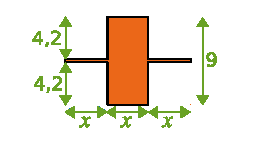
\includegraphics[width=.2\linewidth]{EqQCM01}

\begin{ChoixQCM}{4}
\item Le périmètre de la figure est, en fonction de $x$ : $3x + 9$
\item On peut trouver $x$ pour que la figure  ait le même périmètre qu'un carré de côté $x$
\item Pour la figure, l'équation $6x + 18 = 10,2x$ a un sens
\item L'aire de la figure est en fonction de $x$ : $10,2x$
\end{ChoixQCM}

\begin{corrige}
\reponseQCM{a}
\end{corrige}
\end{exercice}



\begin{exercice}
$a - b$ est négatif ou nul donc...
\begin{ChoixQCM}{4}
\item $a$ peut être égal à $b$
\item $a$ et $b$ sont négatifs
\item $a < b$
\item $a$ est inférieur ou égal à $b$
\end{ChoixQCM}

\begin{corrige}
\reponseQCM{a}
\end{corrige}
\end{exercice}





\begin{exercice}
$x < y$ donc...
\begin{ChoixQCM}{4}
\item $12x < 12 y$
\item $-x < -y$
\item $2x - 5 > 2y - 5$
\item $x^{-1} < y^{-1}$
\end{ChoixQCM}

\begin{corrige}
\reponseQCM{a}
\end{corrige}
\end{exercice}





\begin{exercice}
$4x + 3 < 9$ donc...
\begin{ChoixQCM}{4}
\item $4x > 9 - 3$
\item $\dfrac{4x+3}{9}< 1$
\item $x$ peut être égal à 10
\item $x < 1,5$
\end{ChoixQCM}

\begin{corrige}
\reponseQCM{a}
\end{corrige}
\end{exercice}



\begin{exercice}
$5,6 < c < 8,1$ donc...
\begin{ChoixQCM}{4}
\item $c - 8,5 > 0$
\item la circonférence d'un cercle de rayon $c$ est comprise entre $11,2\pi$ et $16,2\pi$ 
\item le périmètre d'un rectangle de dimensions $c$ et$3c$ est compris entre 44,8 et 64,8
\item $3c-5$ peut être égal à 10,9
\end{ChoixQCM}

\begin{corrige}
\reponseQCM{a}
\end{corrige}
\end{exercice}


\end{GroupeQCM}
\end{QCM}